% Journal-style manuscript fragment for insertion into the shared manuscript.
% Insert the first subsection under Results and the second under Methods.

\subsection{Integration reveals an unfavorable multidimensional SOKM trade-off}
\label{sec:integration-tradeoffs}

Frozen Youth, Identity, and Risk outputs were integrated at the biological-unit
level to assess whether SOKM induced a jointly favorable regenerative state.
The primary profile comprised Youth M1, background-corrected primary Identity,
Pluripotency Risk, and Genomic Stress Risk; Youth M4 and rank-based Identity
were retained as sensitivity outputs. All scores were available for the same 18
animal-level units. Because the modules quantify distinct biological
properties on non-equivalent scales, the axes were analyzed separately rather
than combined into a composite score.

The cross-axis association structure indicated that Youth, Identity, and Risk
were related but non-redundant (Fig.~\ref{fig:mashiro-correlation}). Youth M1
was moderately associated with primary Identity (Spearman $\rho=0.498$;
bootstrap 95\% CI, $-0.006$ to $0.813$; Benjamini--Hochberg-adjusted
$q=0.051$). Youth M1 was inversely associated with Genomic Stress Risk
($\rho=-0.598$; 95\% CI, $-0.860$ to $-0.126$; $q=0.019$), whereas its
association with Pluripotency Risk was weaker and more uncertain
($\rho=-0.385$; 95\% CI, $-0.700$ to $0.168$; $q=0.139$). Thus, similarity
to the young MSC reference was associated with, but did not substitute for,
preservation of MSC Identity or direct evaluation of Risk.

Primary Identity was strongly inversely associated with both Risk programs.
The corresponding correlations were $\rho=-0.748$ for Pluripotency Risk
(95\% CI, $-0.892$ to $-0.389$; $q=0.002$) and $\rho=-0.820$ for Genomic
Stress Risk (95\% CI, $-0.956$ to $-0.504$; $q<0.001$). These relationships
persisted after adjustment for Youth M1, age group, and exact treatment arm,
with partial rank correlations of $-0.607$ and $-0.782$, respectively. Youth
M1 alone accounted for approximately 25\% of the rank-scale variation in
primary Identity. Identity therefore contributed information beyond the Youth
axis rather than functioning as a mathematical correction to it.

The two Risk programs were highly correlated ($\rho=0.858$), and their
association remained substantial after centering within age-by-treatment
strata ($\rho=0.750$) and after adjustment for age and exact treatment arm
(partial rank correlation $=0.731$). Nevertheless, the programs did not
produce identical donor rankings. Pluripotency Risk and Genomic Stress Risk
were therefore retained as correlated but biologically distinct coordinates;
the results do not support strict statistical independence or replacement by a
single undifferentiated Risk measure.

\begin{figure*}[t]
\centering
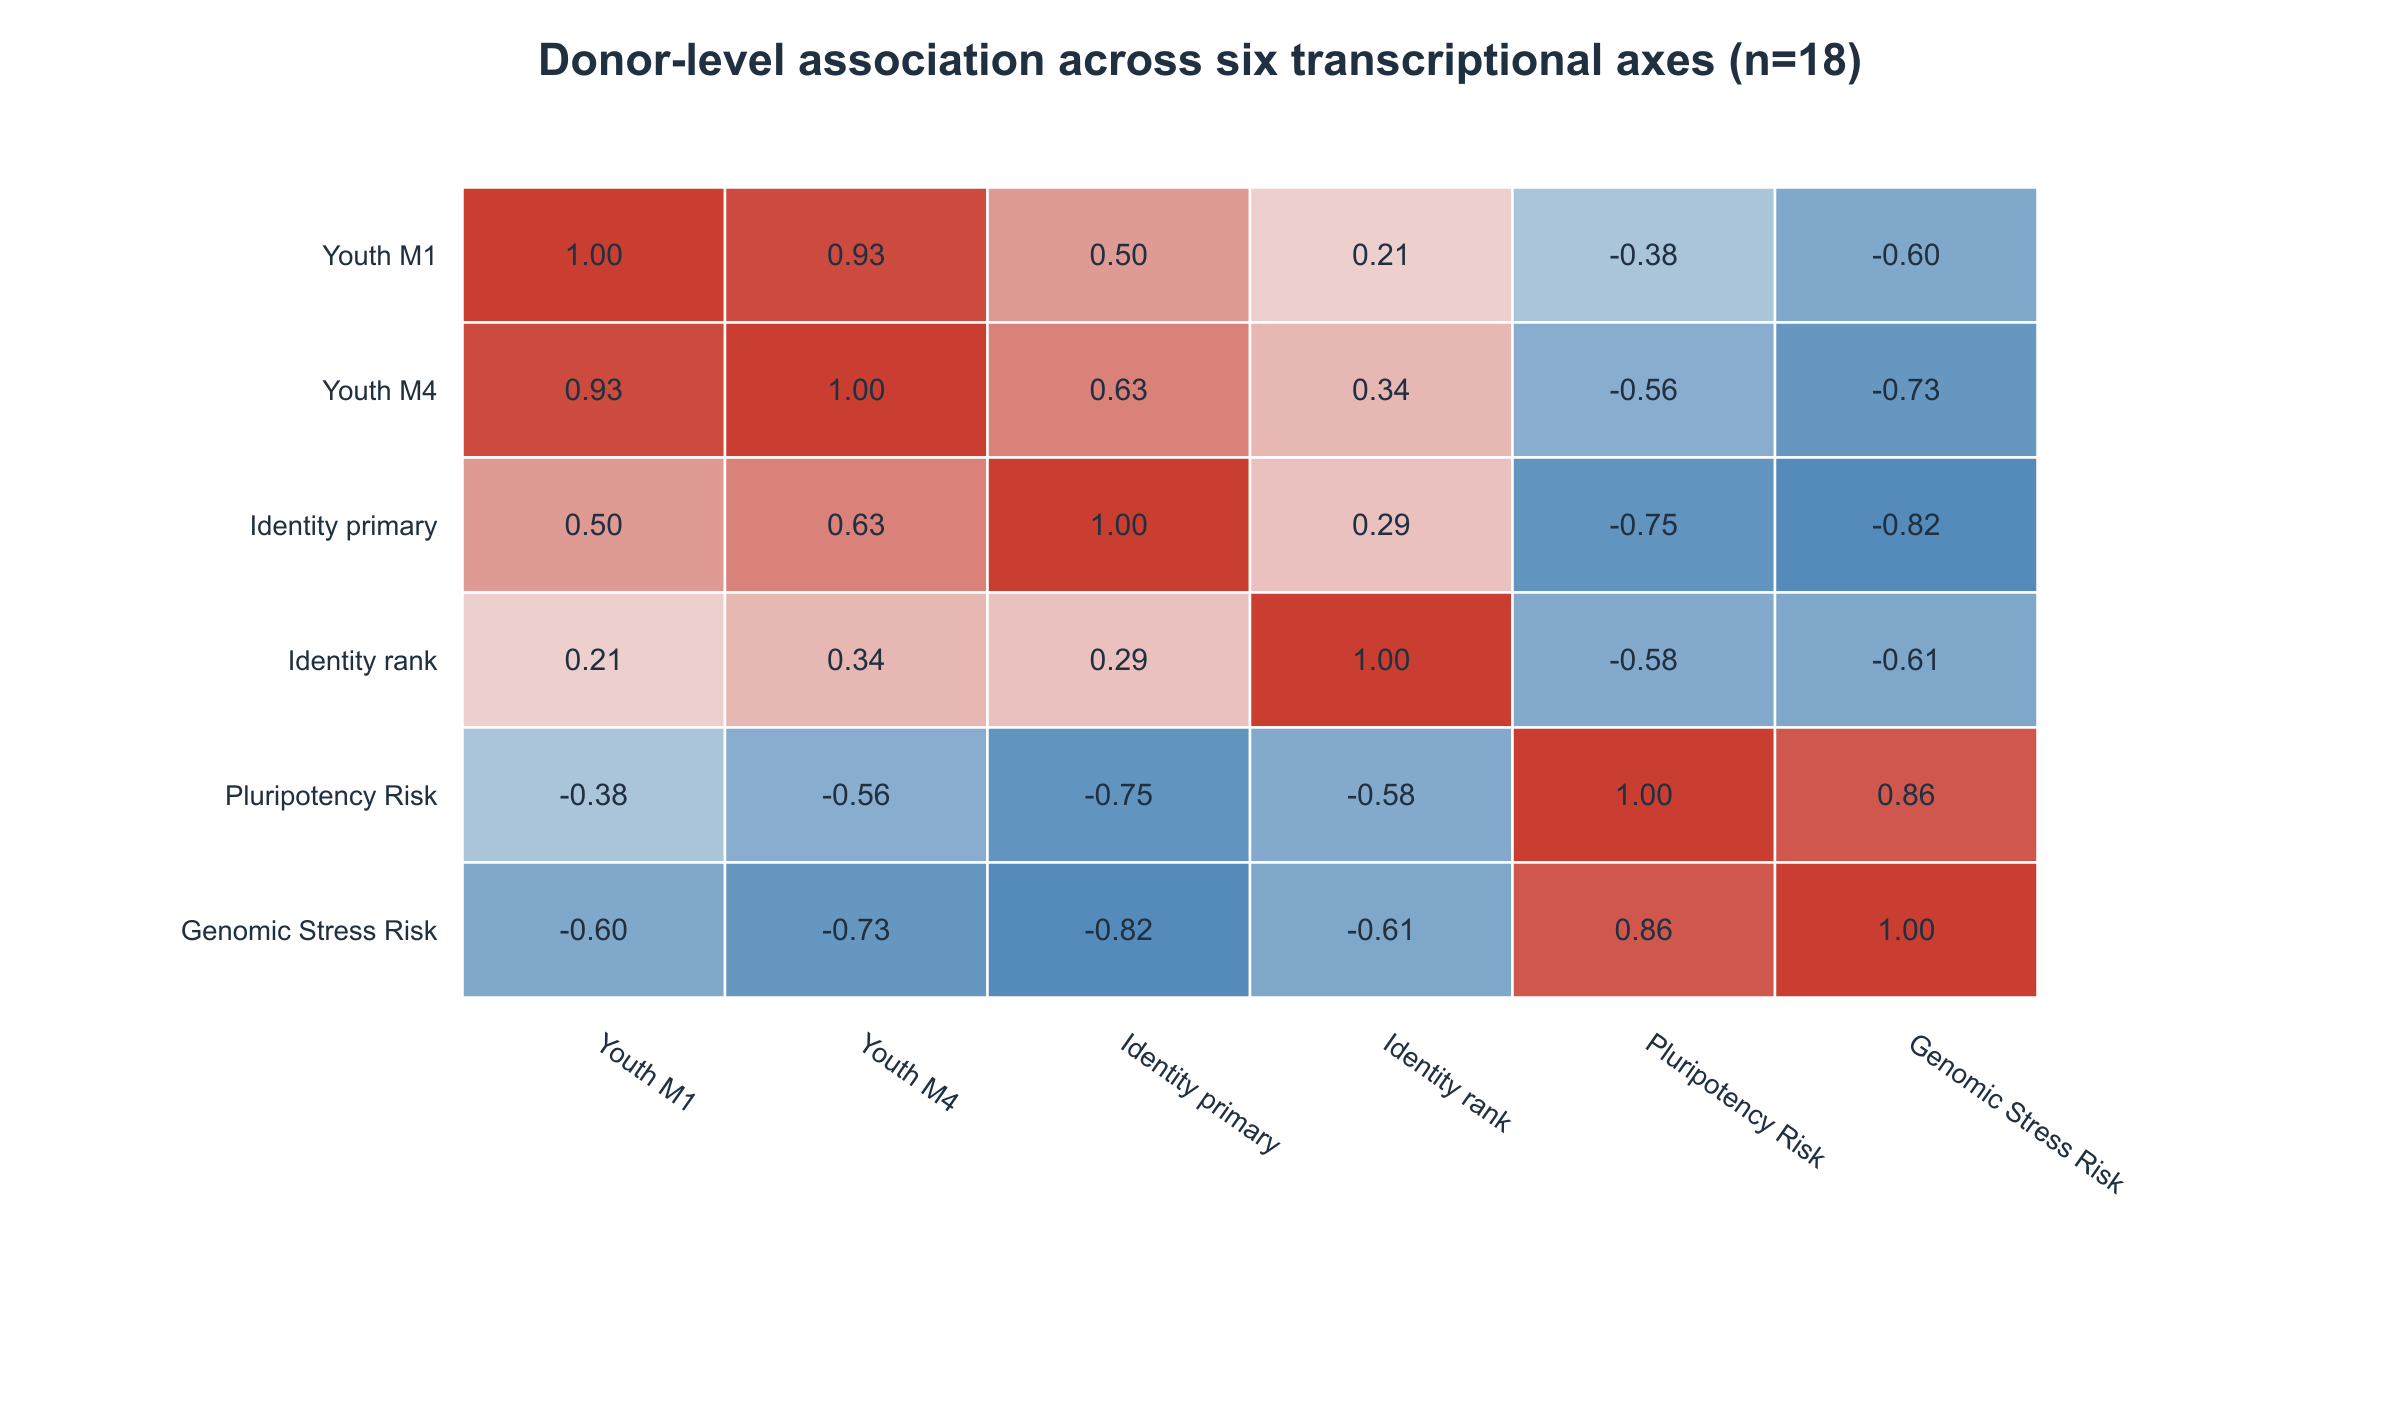
\includegraphics[width=0.88\textwidth]{figures/mashiro_six_axis_heatmap.png}
\caption{Association structure across frozen Youth, Identity, and Risk
outputs. Values are Spearman correlations across 18 unpaired animal-level
biological units. Youth M1 and primary Identity were the prespecified primary
outputs; Youth M4 and rank-based Identity were sensitivity outputs. The matrix
describes association and does not imply interchangeability or causal
dependence.}
\label{fig:mashiro-correlation}
\end{figure*}

Agreement between the primary and sensitivity Youth models was high
($\rho=0.930$). By contrast, primary and rank-based Identity showed modest
agreement ($\rho=0.286$), consistent with their distinct definitions of
expression-matched enrichment and within-cell rank prominence. The
background-corrected score was therefore retained for the prespecified primary
integration, while rank-based Identity was treated as a separate sensitivity
analysis rather than used to replace the primary result on the basis of the
observed treatment contrast.

Age-specific comparisons showed a consistent multidimensional SOKM pattern
(Table~\ref{tab:mashiro-safe-zone}). SOKM was compared separately with each
exact control arm within young and aged animals. The median SOKM-minus-control
difference in Youth M1 was negative in all four comparisons. Pluripotency Risk
and Genomic Stress Risk were higher under SOKM in all four comparisons. Primary
Identity was lower in three comparisons and was essentially unchanged in aged
animals relative to the \texttt{Tg-/Dox+} control.

\begin{table*}[t]
\centering
\caption{Age-specific multidimensional SOKM trade-offs. Values are differences
in condition medians between SOKM and the indicated control. The prespecified
favorable directions were Youth M1 $>0$, primary Identity $\geq0$,
Pluripotency Risk $\leq0$, and Genomic Stress Risk $\leq0$. The criteria
constitute a directional screen rather than a validated efficacy or safety
threshold.}
\label{tab:mashiro-safe-zone}
\small
\begin{tabular}{llrrrrc}
\toprule
Age & Control arm & Youth M1 & Identity primary & Pluripotency Risk & Genomic Stress Risk & Criteria met \\
\midrule
Young & \texttt{Tg+/Dox-} & -0.0648 & -0.1335 & 0.0570 & 0.0209 & 0/4 \\
Young & \texttt{Tg-/Dox+} & -0.0787 & -0.0175 & 0.0490 & 0.0161 & 0/4 \\
Aged  & \texttt{Tg+/Dox-} & -0.0148 & -0.1280 & 0.0513 & 0.0229 & 0/4 \\
Aged  & \texttt{Tg-/Dox+} & -0.0400 &  0.0025 & 0.0418 & 0.0123 & 1/4 \\
\bottomrule
\end{tabular}
\end{table*}

A directional trade-off screen was used to summarize the joint pattern without
assigning arbitrary weights across modules. A comparison was considered
favorable only when SOKM showed higher Youth M1, non-decreased primary
Identity, and non-increased values of both Risk programs. None of the four
age-specific comparisons met all four criteria; three met none, and one met
only the Identity criterion. The condition-level map yielded the same overall
interpretation in both age groups (Fig.~\ref{fig:mashiro-map}). SOKM occupied a
region characterized by lower Youth, generally lower Identity, and higher Risk
relative to the exact controls. The plotted control-to-SOKM vectors are
descriptive contrasts between unpaired condition medians and do not represent
within-animal trajectories.

\begin{figure*}[t]
\centering
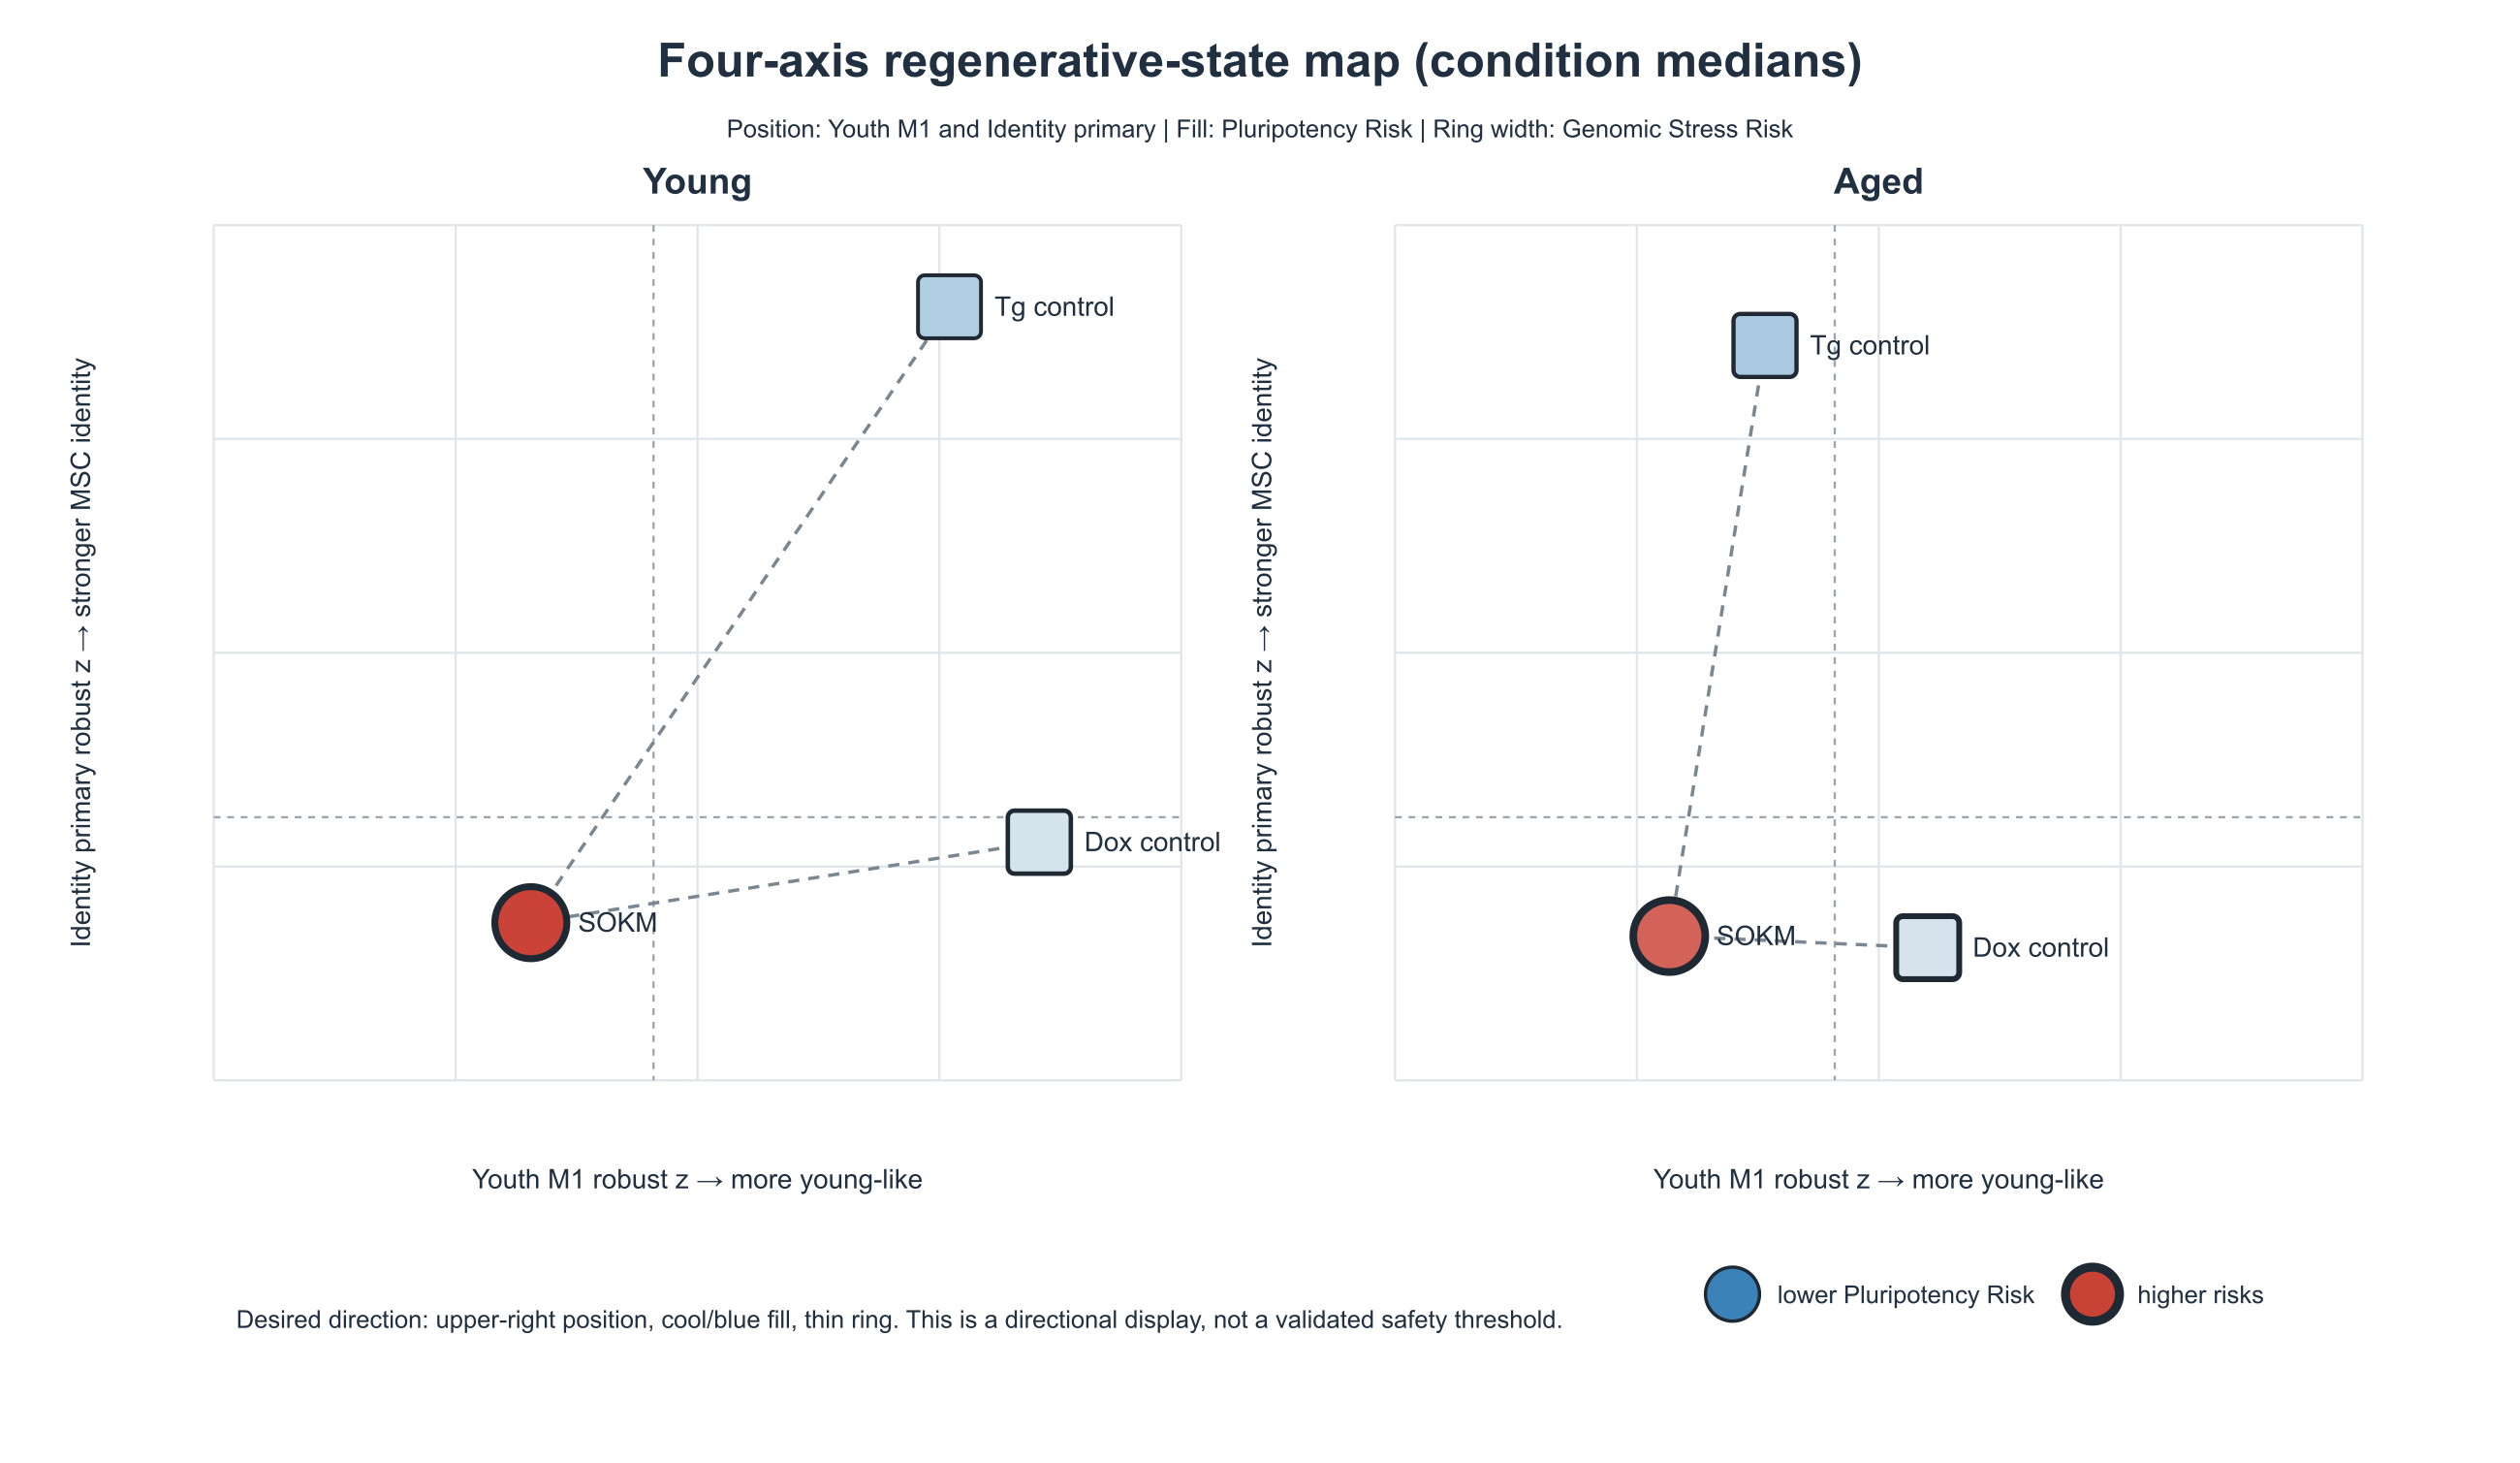
\includegraphics[width=0.96\textwidth]{figures/mashiro_four_axis_map.png}
\caption{Condition-level multidimensional regenerative-state map. Horizontal
and vertical positions represent median Youth M1 and primary Identity after
within-axis robust standardization. Fill represents Pluripotency Risk, and
outline width represents Genomic Stress Risk. Robust standardization was used
for visualization only; the axes were not averaged. Dashed vectors show
descriptive control-to-SOKM differences within each age group and do not imply
paired sampling.}
\label{fig:mashiro-map}
\end{figure*}

The principal associations were robust to prespecified sensitivity analyses.
Exclusion of the three biological units containing fewer than 100 cells did not
reverse the main association patterns. The direction of each of six key
cross-axis correlations was preserved in all 18 leave-one-unit-out analyses.
No age-by-treatment interaction remained significant after correction across
12 exact permutation tests. Given the limited number of biological units per
age-by-arm stratum ($n=3$), the absence of an interaction signal should not be
interpreted as evidence of equivalent effects in young and aged animals.

Collectively, the tested SOKM condition did not satisfy the prespecified
favorable transcriptional pattern of increased Youth, preserved MSC Identity,
and non-increased Pluripotency and Genomic Stress Risk. This finding does not
establish functional impairment, tumorigenicity, or clinical unsafety; it
indicates that the tested condition did not occupy the favorable region of the
defined transcriptional state space. More broadly, the analysis demonstrates
that evaluation of partial reprogramming requires separate consideration of
Youth, Identity, and Risk, because reduction to a single scalar score would
obscure the observed biological trade-offs.


\subsection{Data integration and statistical analysis}
\label{sec:integration-statistics}

Following module-contract harmonization and construction of the canonical
biological-unit table described in Section~4.1, statistical integration was
performed across 18 animal-level units comprising two age groups, three exact
treatment arms, and three animals per age-by-arm stratum. Treatment arms were
analyzed as unpaired. Native module outputs were neither refitted nor
rescaled during integration.

Youth M1, background-corrected primary Identity, Pluripotency Risk, and Genomic
Stress Risk were designated as the primary axes. Youth M4 and rank-based
Identity were prespecified sensitivity outputs. Donor-level median cell scores
were used for both Risk programs in the primary integration; upper-tail Risk
summaries were retained as module-specific supporting analyses. No composite
score was calculated.

Pairwise associations among the six outputs were estimated using Spearman
correlation. Bootstrap 95\% confidence intervals were obtained from 10,000
biological-unit resamples. Two-sided nominal $p$-values were estimated from
20,000 permutations, and the 15 pairwise comparisons were adjusted using the
Benjamini--Hochberg procedure. Because the study included a small number of
independent biological units, these analyses were considered exploratory.

SOKM (\texttt{Tg+/Dox+}) was compared separately with
\texttt{Tg+/Dox-} and \texttt{Tg-/Dox+} within each age group. For each axis,
unpaired differences in group medians and means and Cliff's delta were
calculated. The control arms were not pooled. Condition-level robust $z$ scores
were calculated independently within each primary axis for visualization and
were not used to derive a combined endpoint.

The directional trade-off screen classified a comparison as favorable when
the SOKM-minus-control median differences simultaneously satisfied Youth M1
$>0$, primary Identity $\geq0$, Pluripotency Risk $\leq0$, and Genomic Stress
Risk $\leq0$. The rule assessed direction only and was not interpreted as a
validated biological threshold. Partial rank correlations were used to assess
associations between Identity and each Risk program after adjustment for the
corresponding Youth output, age group, and exact treatment arm. Rank-scale
linear models were additionally used to estimate the fraction of Identity
variation explained by Youth alone and by Youth together with the design
variables.

Overlap between the two Risk programs was evaluated using overall Spearman
correlation, Spearman correlation after age-by-arm mean centering, and partial
rank correlation adjusted for age and exact treatment arm. Robustness analyses
were conducted after exclusion of biological units with fewer than 100 cells,
after omission of each biological unit in turn, and separately within each age
group. Exploratory age-by-treatment interactions were calculated separately
for each control arm as the difference between aged and young mean SOKM
effects. Two-sided exact permutation $p$-values were obtained from all 400
age-label assignments that preserved three aged and three young samples within
each treatment arm, followed by Benjamini--Hochberg correction across 12
interaction tests.

All statistical analyses treated animal-level biological units, rather than
individual cells, as independent observations. The integrated analysis
evaluated transcriptional state coordinates and did not directly assess
functional rejuvenation, tumor formation, or clinical safety.
